\chapter[Forschungsfrage 1]{Wie können Container-Anwendungen den Prozess des automatisierten \enquote{Deployments} unterstützen?} \label{ff1}
Kapiteleinleitung...

\section{Grundlagen: Definieren der Begrifflichkeiten zur Forschungsfrage eins}
Dieses Kapitel soll grundlegende Begrifflichkeiten, die im weiteren Verlauf dieser Arbeit verwendet werden, definieren, um so eine einheitliche Terminologie der Begriffe zu entwickeln. Dadurch wird ein gemeinsames Verständnis erzeugt.

\subsection{Methodik der Anforderungsanalyse}
Die Anforderungsanalyse leitet sich aus dem thematischen Komplex des \enquote{Requirements-Engineering} ab, die verschiedene Bedeutungsvarianten besitzt -- dabei \enquote{[...] steht [es] einmal für alle konkreten Aktivitäten am Beginn einer Systementwicklung, die auf eine Präzisierung der Problemstellung abzielen. Ebenso steht es aber auch für eine ganze Teildisziplin im Grenzbereich zwischen Systems-Engineering, Informatik und Anwendungswissenschaften.}\autocite[][S.19]{partsch_requirements-engineering_2010} Diese Analyse soll, laut der herrschenden Meinung der Wissenschaft, am Anfang jeder Systementwicklung stehen, um so bestimmte Vorgehensweise anzuwenden. Dabei entstehen, wenn der später weiter definierte Prozess verfolgt wird, viele systematisch verbundene Dokumente, die Anforderungen enthalten. So ist jede Anforderung wieder ein Cluster von kleineren Anforderungen, die miteinander verbunden sind. Diese werden durch den IEEE-Standard 1220 definiert als \enquote{a statement that identifies a product or process operational, functional, or design characteristic or constraint, which is unambiguous, testable or measurable, and necessary for product or process acceptability (by consumers or internal quality assurance guidelines).}\autocite[][S.9]{IEEE1220-2005SystemsEng} Dieser Standard legt mit höchster Priorität den Fokus auf die Formulierung einer Anforderung als elementar wichtig für das Produkt bzw. für das Erreichen der Akzeptanz des Produktes. Ziel der Analyse ist es, funktionale und nicht-funktionale Anforderungen zu identifizieren und diese testbar zu dokumentieren. Funktionale Anforderungen definieren genau, was ein System später erfüllen muss, sie ergeben sich aus der Fragestellung \enquote{Was tut das System?/Was soll es aufgrund der Aufgabenstellung können?}\autocite[][S.27]{partsch_requirements-engineering_2010} Nicht-funktionale Anforderungen konkretisieren die Qualitätsansprüche an das System, die Forderung an das zu implementierende System als Ganzes, sowie Randbedingungen, die aus Projekt-/Prozess-/Unternehmensbedingungen resultieren können.\autocite[vgl.][S.27-29]{partsch_requirements-engineering_2010}

\begin{figure}[H]
	\centering
	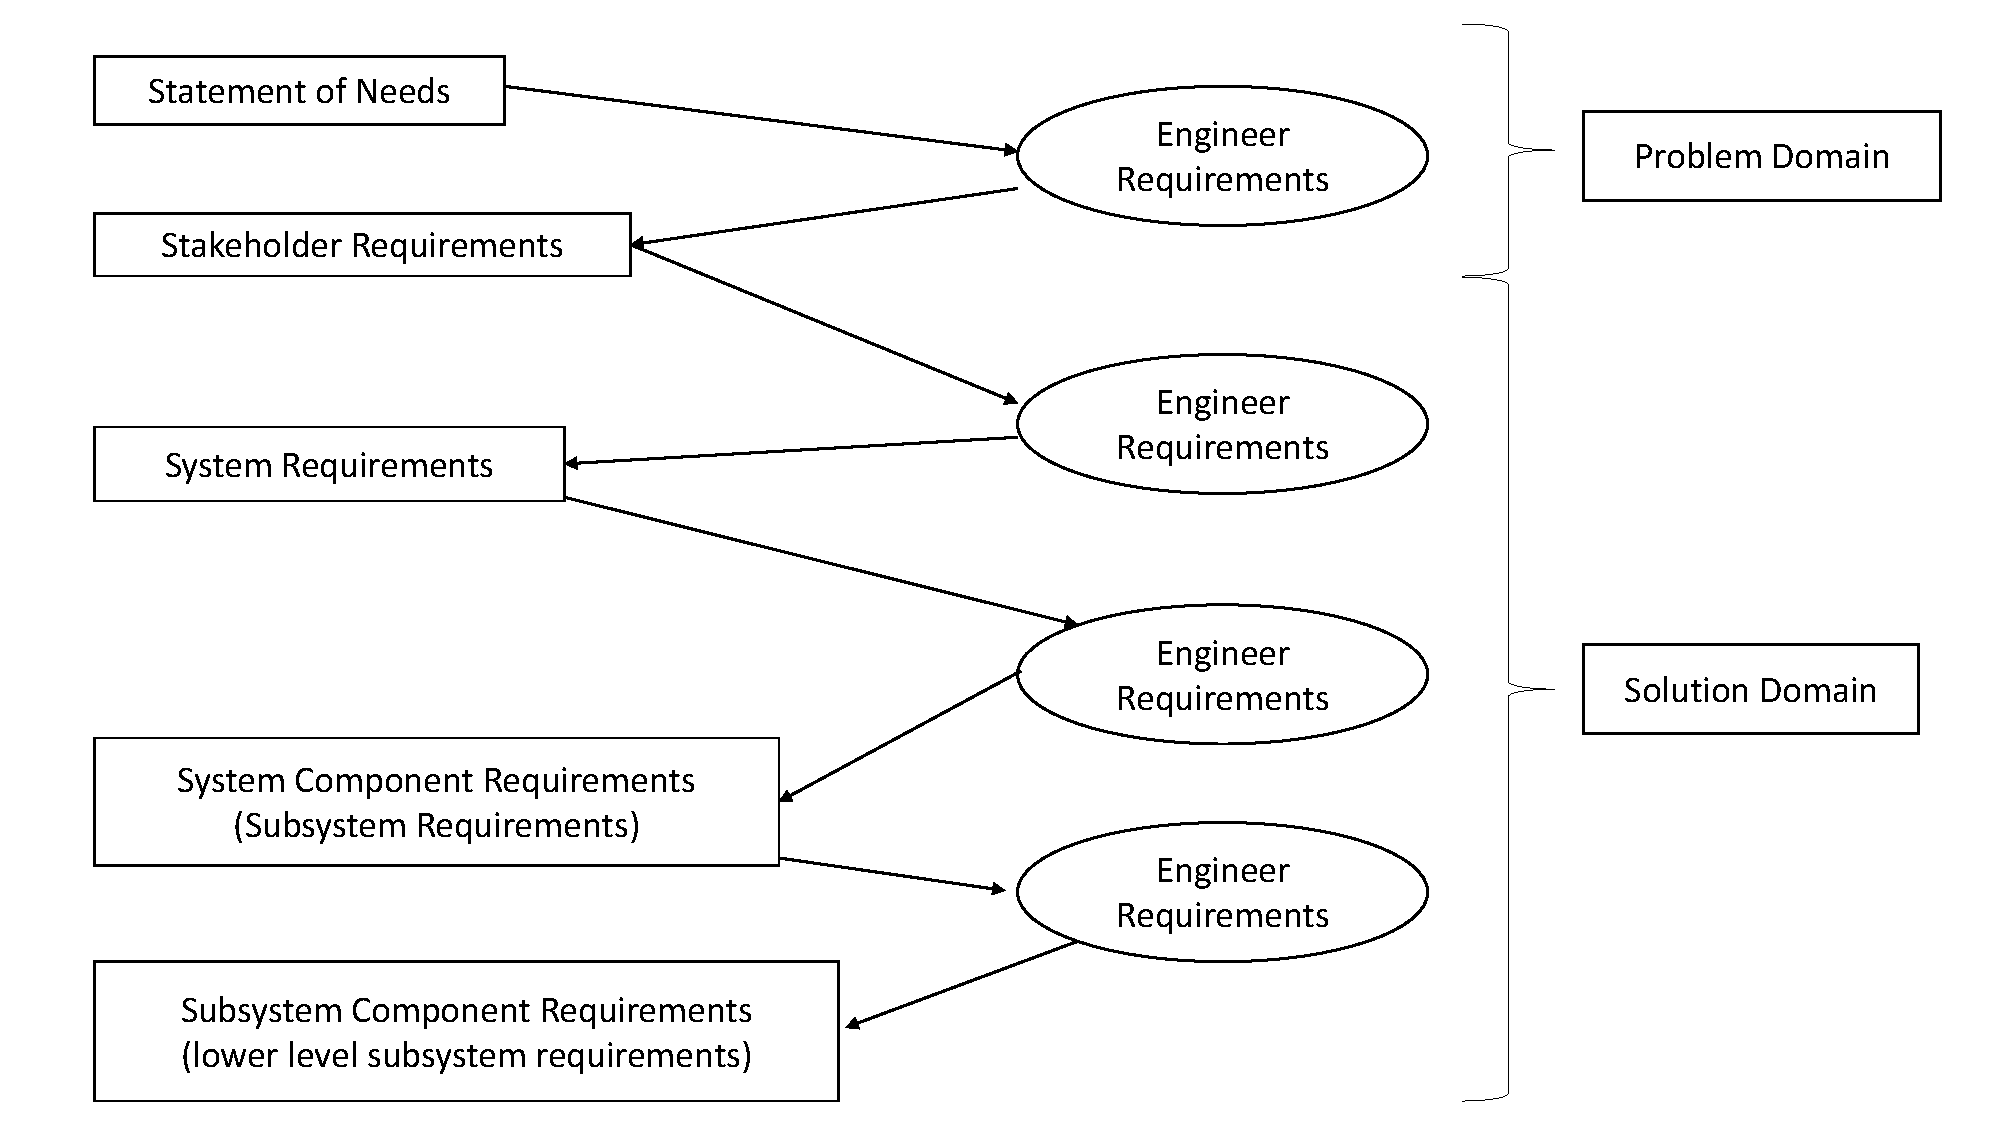
\includegraphics[scale=0.38]{img/levels-of-requirements-engineering.pdf}
	\caption{Entwicklungsprozess der Anforderungen}
	{\footnotesize \cite[Quelle: in Anlehnung an ][S.28]{hull_requirements_2011}}
	\label{abb:entwAnforderung}
	%		{\scriptsize \textit{Alle Rechte, einschließlich der Vervielfältigung, Veröffentlichung, Bearbeitung und Übersetzung bleiben der SV Informatik GmbH vorbehalten.}}
\end{figure}

Das \enquote{Statement of Needs} ist der Startpunkt für die Entwicklung einer Anforderung die am Ende des Prozesses, der in Abbildung \vref{abb:entwAnforderung} dargestellt ist, präzise dokumentiert sein wird. Dieses ist am Anfang immer ein Ausdruck eines Anspruchs oder Wunsches an das zu entwerfende System; dabei bildet es und die \enquote{text} 

\subsection{Cloud Computing}

\subsection{Container}

\subsection{\enquote{Deployment}} \label{defDeployment}

\section{Ist-Analyse des jetzigen \enquote{Deployment}-Prozesses}

\section{Konzeption eines container-basierten, automatisierten \enquote{Deployments}}